\chapter{Scope rules}\label{chap:scope-rules}
This section describese scope rules and the environment-store model for the language. It is important to know how the values of variables are being stored as well as knowing how the language handles encapsulation. 

\section{The environment-store model}\label{sec:es-model}
The environment-store model is important to know how works. This is because the model describes how variables values are stored, and what variable is bound to a certain location. Furthermore it also describes what value a location has stored. Figure \ref{fig:esmodel}, illustrates the environment-store model. The model shows three boxes. The left box is the environment, the middle is the location and the right is the store. The environment is where variables are. A variables is bound to a location, which is illustrated by the arrow, $env_v$ (variable-environment). $env_v$ is a function retrieves the location of a variable. On a location, the value of the variable can be stored, which is illustrated by the $sto$ arrow. $sto$ is a function that retrieves the value stored on a location. 
\\For example, the model shows that the variable $x$ is bound to location 25, which has the value $5$ stored. The same is valid for the variables $y$ and $z$. However these two variables are bound to the same location, which has the same value stored. If for example, the value 13 in store, gets changed to 15, then the value for both variables $y$ and $z$ changes. 
\begin{figure}[H]
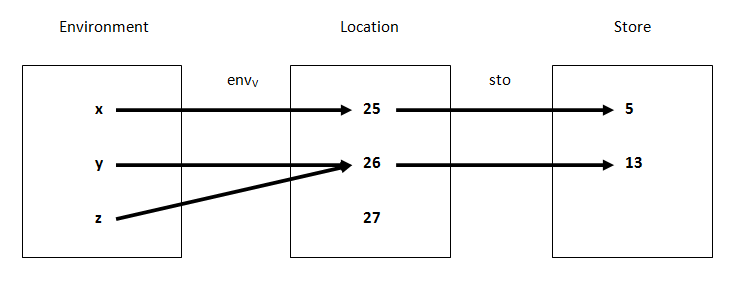
\includegraphics{billeder/environment_store_model.png}
\caption{Environment-store model}
\label{fig:esmodel}
\end{figure}


\section{The scope rules}\label{sec:scope-rules}




\begin{center}
\begin{tabular}{ l l}
\hline
& \\
$[CALL-STAT-STAT_{BSS}]$ & $env'_{v}~[next \rightarrow l], env'_{p}~ \vdash \langle S,sto \rangle \rightarrow sto' \over env_{v}, ~ env_{p} \vdash \langle call~p, sto \rangle \rightarrow sto'$ \\
& where $env_{p}p = (S,env'{v},env'{p})$ \\
& and $l = env_{v}next$ \\
\hline
\end{tabular}
\end{center}







